\subsection{Log GLSM invariants}%
\label{sub:Log GLSM invariants}

\begin{defn}
    We will define the \textit{decorated tropical type} of a log map \(f\) as
    \[ \bm{\tau} = (G, c \colon \H \to \Z, \beta \colon \V \to H_2(X)). \]
\end{defn}

\begin{defn}
    A log or punctured map \(f\) is of \textit{compact type} if
    \begin{enumerate}
        \item \(\Ima \Sigma(f)_t\) is bounded for all \(t\);
        \item \(f(p_h) \in 0_{\mf{P}}\) for all half-edges \(h\) with contact order \(0\).
    \end{enumerate}
\end{defn}

We are now able to define the category \(\mc{R}(\mf{P}, \tau)\) of stable punctured R-maps fibered over the category \(\ms{LogSch}\) of fs log schemes and marked by \(\tau\).

\begin{thm}[{\cite{CJR2021,CJRpunctured}}]
    The stack \(\mc{R}(\mf{P},\bm{\tau})\) is represented by a proper DM stack with basic/minimal log structure.
\end{thm}

\begin{rmk}
    If \(\V = \ab\{v\}\) is a singleton, then we will write
    \[ \mc{R}_{g, c}(\mf{P}, \beta) \coloneqq \mc{R}(\mf{P}, \bm{\tau}). \]
\end{rmk}

Consider the diagram
\begin{equation*}
\begin{tikzcd}
    & \mf{P} \ar{d} \\
    \mc{C} \ar{ur}{f} \ar{d}{\pi} \ar{r} & B \C_{\omega}^{\times} \\
    \mc{R},
\end{tikzcd}
\end{equation*}
where we set \(\mc{R} \coloneqq \mc{R}(\mf{P}, \bm{\tau})\). Then the perfect obstruction theory is defined by
\[ T_{\mc{R}/\ms{Log}_{\mf{M}_G}} \to \E_{\square} = R \pi_* f^* T_{\mf{P}/B\C_{\omega}^{\times}}. \]
Here, both tangent bundles refer to the log tangent complex. From the perfect obstruction theory, this defines the canonical virtual cycle
\[ [\mc{R}(\mf{P}, \bm{\tau})]^{\vir}. \]
The main drawback of this virtual cycle is that it does not reproduce Gromov-Witten theory. However, we can consider how it differs from GW theory, but for this we need a birational modification. Let \(Q\) be a sharp monoid. It has a partial ordering by \(a < b\) if there exists a nonzero \(c \in Q\) such that \(a+c = b\).

\begin{defn}
    We say that either \(f\)  or \(\Sigma(f)\) has \textit{uniform maximal degeneracy} if there exists \(e_{\max} \in \ab\{e_v \mid v \in \V \}\) such that \(e_{\max} \geq e_v\) for all \(v \in \V\).
\end{defn}

\begin{rmk}
    If \(f\) is compact type and has uniform maximal degeneracy, then \(\Sigma(f)\) is uniformly bounded by \(e_{\max}\).
\end{rmk}

\begin{defn}
    Define \(\mc{U}(\mf{P}, \bm{\tau})\) to be the stack of stable punctured or log R-maps marked by \(\bm{\tau}\) with uniform maximal degeneracy.
\end{defn}

\begin{rmk}
    If \(\V = \ab\{v\}\) is a singleton, then we will write
    \[ \mc{U}_{g, c}(\mf{P}, \beta) \coloneqq \mc{U}(\mf{P}, \bm{\tau}). \]
    If one of the contact orders is negative, then we will write
    \[ \mc{U}_{g, c}(\infty, \beta) \coloneqq \mc{U}(\mf{P}, \bm{\tau}). \]
\end{rmk}

Note that there are two types of vertices: if a vertex is mapped to \(0\), then either there is at least one half-edge which points upwards or all contact orders are \(0\), in which case all are contracted. These are called \textit{log vertices}. The other type of vertex is one that does not go to \(0\). Either all half-edges point downwards, or there are some half-edges which point upwards. These are called \textit{\(\infty\)-vertices}. Moreover, the vertices which are compact types are the ones without upwards-pointing half-edges.

If we forget the condition of having uniform maximal degeneracy, then there is a map
\[ \mc{U}(\mf{P}, \bm{\tau}) \xrightarrow{F} \mc{R}(\mf{P}, \bm{\tau}) \]
which is a subcategory over \(\ms{LogSch}\). However, as a morphism of algebraic stacks, it is log \'etale, proper, and surjective. In addition, \(\mc{U}\) has a canonical perfect obstruction theory which is pulled back from \(\mc{R}\). In the case when the set of vertices is a singleton, we have
\begin{align*}
    F_* [\mc{U}_{g, c}(\mf{P}, \beta)]^{\vir} &= [\mc{R}_{g, c}(\mf{P}, \beta)]^{\vir}; \\
    F_* [\mc{U}_{g, c}(\infty, \beta)]^{\vir} &= [\mc{R}_{g, c}(\infty, \beta)]^{\vir}.
\end{align*}
In the case of a log vertex, we in fact have inclusions from the moduli of stable maps with p-fields as
\begin{equation*}
\begin{tikzcd}
    \mc{U} \ar{rr}{F} & & \mc{R} \\
    & \mc{R}_{g,c}(\mf{P}^{\circ}, \beta) \ar[hookrightarrow]{ul} \ar[hookrightarrow]{ur}.
\end{tikzcd}
\end{equation*}
If we denote the moduli of p-fields by \(\mc{R}^{\circ}\), then the boundary
\[ \Delta \coloneqq \mc{U} \setminus \mc{R}^{\circ} \]
is a Cartier divisor. By the condition of having uniform maximal degeneracy, we have a section
\[ e_{\max} \in H^0(\bar{M}_{\mc{U}}). \]
This is equivalent to the data of a morphism
\[ \mc{U} \to ([\A^1/\G_m], 0) \]
which pulls \(0\) back to \(\Delta\).

We will define a \textit{superpotential} to be a function
\begin{equation*}
\begin{tikzcd}
    \mf{P}^{\circ} \ar{rr}{W} \ar{dr} && \mc{L}_{\omega} \ar{dl} \\
    & B \C_{\omega}^{\times}.
\end{tikzcd}
\end{equation*}
Its \textit{critical locus} is denoted by 
\[ \on{Crit}(W) = (\d{W} = 0). \]
We say that \(W\) has \textit{proper critical locus} if \(\on{Crit}(W) \to B\C_{\omega}^{\times}\) is proper.

For example, suppose we are interested in GW theory. Let \(X\) be a smooth projective variety, \(V\) be a vector bundle on \(X\), and \(s \in H^0(V)\). Set \(Z = (s = 0)\). Then we obtain
\[ W \colon \mf{P}^{\circ} = V^{\vee} \boxtimes \mc{L}_{\omega} \xrightarrow{s \otimes 1_{\omega}} \mc{L}_{\omega}. \]

\begin{lem}
    \(W\) has proper critical locus if and only if \(Z\) is smooth of expected codimension.
\end{lem}

\begin{exm}
    Let \(X\) be a point, \(V = \C\), and \(s \neq 0\). Then \(\d{W} = s \neq 0\), so the critical locus is empty.
\end{exm}

Using the Kiem--Li method of cosection localization~\cite{KiemLi2013}, we can obtain a virtual cycle
\[ [\mc{R}_{g, c=n}(\mf{P}^{\circ}, \beta)]_W^{\vir}, \]
which is supported on the critical locus. In GW theory, this equals the GW virtual cycle, 
\[ \pm [\bar{M}_{g,n}(\on{Crit}(W), \beta)]^{\vir}, \]
where the sign can be explicitly calculated.

\begin{thm}[{\cite{CJR2021,CJW2021}}]
    Let \(\bm{\tau}\) be of compact type. In the compact type setting, 
    \begin{enumerate}
        \item \(\mc{U}(\mf{P}, \bm{\tau})\) has a reduced perfect obstruction theory, which yields a reduced virtual cycle \([\mc{U}(\mf{P}, \bm{\tau})]^{\vir}\);
        \item \(\Delta\) has a reduced perfect obstruction theory, which yields a reduced virtual cycle \([\Delta]^{\vir}\);
        \item We have \([\mc{U}_{g, c=n}(\mf{P}, \beta)]^{\on{red}} = \pm [\bar{M}_{g,n}(\on{Crit}(W), \beta)]^{\vir}\) in the case of a single log vertex. Moreover, there is the formula
            \[ [\mc{U}_{g, c=n}(\mf{P}, \beta)]^{\on{red}} = [\mc{U}_{g, c=n}(\mf{P}, \beta)]^{\vir} - \tilde{r} [\Delta]^{\on{red}}, \]
            where \(\tilde{r}\) is the pole order of \(W\) along \(\infty\).
    \end{enumerate}
\end{thm}

\subsection{Tropical decomposition and finite generation}%
\label{sub:Tropical decomposition and finite generation}

The tropical decomposition and its applications below are from the working draft~\cite{CJRtropical2025}. The effective invariants and their axioms are developed in~\cite{CJRpunctured}.

From now on, we will consider a simpler setup where \(X\) is a smooth projective variety and \(V\) is a line bundle on \(X\). In this case, we will assume that \(Z = (s = 0)\) is smooth of codimension \(1\). Moreover, we will assume that \(Z\) is a Calabi-Yau threefold. We will consider the invariants
\[ N_{g, \beta} \coloneqq \int_{[\bar{M}_{g,0}(Z, \beta)]^{\vir}} 1 \in \Q \]
and the generating series
\[ F_g = \sum_{\beta \geq 0} N_{g, \beta} Q^{\beta} \in \Lambda \coloneqq \C \ps{Q}. \]

\begin{conj}[Yamaguchi-Yau, Alim-L\"ange {\cite{YY2004,AlimLange2007}}]
    Suppose \(g=0\) mirror symmetry holds for \(Z\). Then there exists a finitely-generated \(\Q\)-algebra \(R \subset \Lambda\) such that for all \(g \geq 2\), \(F_g \in (I_0(q))^{2g-2} R\).
\end{conj}

Our main goal is the following.

\begin{thm}[{\cite{CJRtropical2025}}]
    Let \(Z\) be a Calabi-Yau threefold hypersurface in a Fano fourfold \(X\) with no odd cohomology. Let \(\{\phi_j\}\) be a basis of \(H^*(X)\) and \(\ab\{\phi^j\}\) be the dual basis. Then for all \(g \geq 0\), we have
    \begin{align*}
        &F_g = (-1)^{1-g} \sum_{\tau' \in G_g'} \frac{(-1)^{\abs{\V_{\infty}}}}{\abs{\Aut(\tau')}} \cdot \prod_{E \in \E} c(E) \\
        & \cdot \sum_{j_E \mid E = \ab\{E_{\log}, E_{\infty}\} \in \E} \prod_{\substack{v \in \V_{\infty} \\ g(v)=1 \\ \H_v = \ab\{E_{\infty}\}}} c_1^{\mr{eff}}(\phi^{j_E}) \cdot \prod_{\substack{v \in \V_{\infty} \\ g(v) \geq 2}} \tilde{Q}^{\beta(v)} \cdot \exp \ab(\int_{\beta(v)} K(Q) )  \\
        & \cdot \ab(\prod_{E_{\infty} \in \H_v'}\int_{\beta(v)} \phi^{j_E}) \cdot c_{g(v), \beta(v)}^{\on{eff}} 
         \cdot \prod_{v \in \V_{\log}} \Omega_{g(v), \abs{\H_1(v)}, \abs{\H_2(v)}} (\phi_{j_E} \colon E_{\log} \in \H_1(v)).
    \end{align*}
\end{thm}

\begin{exm}
    Let \(Y\) be a toric variety with its toric log structure. Then \(\Sigma(Y)\) is the toric fan treated as a cone complex, and we can consider its boundary \(\Delta_Y = \sum_{\rho \in \Sigma(Y)^1} \Delta_{\rho}\). 
\end{exm}

If we consider \([\Delta]^{\on{red}}\), we should obtain the similar formula
\[ [\Delta]^{\on{red}} = \sum_{\rho \in \Sigma(\Delta)(1)} [\Delta_{\rho}]^{\on{red}}. \]
The question now is what the \(\rho\) represent. In fact, they parameterize rigid tropical curves. In the tropicalization
\begin{equation*}
\begin{tikzcd}
    \Sigma(C)_{\rho} \ar{d} \ar{r} & \Sigma(\mc{C}) \ar{r}{f} \ar{d} & \R_{\geq 0} \\
    \rho \ar[hookrightarrow]{r} & \Sigma(\mc{U}),
\end{tikzcd}
\end{equation*}
we see that \(f_{\rho}\) is rigid if and only if the source tropical curve is a bipartite graph with one set of vertices going to \(e_{\max}\) and the other set of vertices going to \(0\).

\begin{exm}
    Let \(X\) be a point and \(Z = \emptyset\). Also consider \(g = 2, n = 0\). Then the possible graphs are given in~\Cref{fig:tropgraphs}.
    \begin{figure}[htpb]
    \begin{center}
    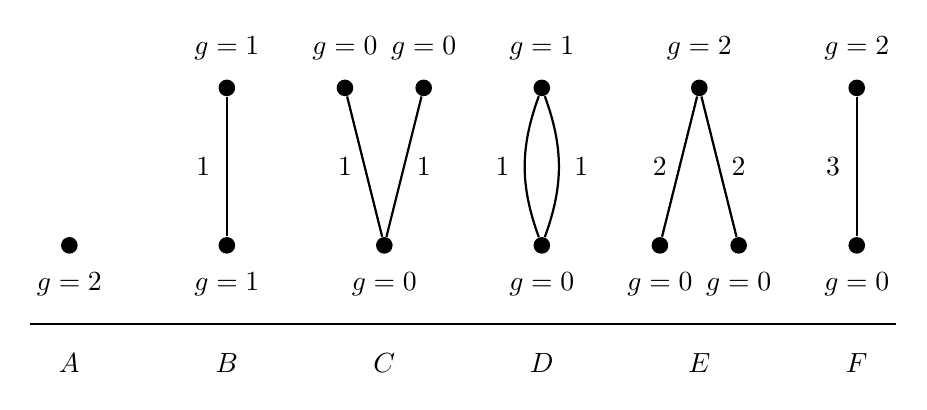
\begin{tikzpicture}[scale=1, transform shape]
        \node[fill=black,circle,minimum size=6pt,inner sep=0pt] (A) at (0,0) {};
        \node[fill=black,circle,minimum size=6pt,inner sep=0pt] (B1) at (2,0) {};
        \node[fill=black,circle,minimum size=6pt,inner sep=0pt] (B2) at (2,2) {};
        \node[fill=black,circle,minimum size=6pt,inner sep=0pt] (C1) at (4,0) {};
        \node[fill=black,circle,minimum size=6pt,inner sep=0pt] (C2) at (3.5,2) {};
        \node[fill=black,circle,minimum size=6pt,inner sep=0pt] (C3) at (4.5,2) {};
        \node[fill=black,circle,minimum size=6pt,inner sep=0pt] (D1) at (6,0) {};
        \node[fill=black,circle,minimum size=6pt,inner sep=0pt] (D2) at (6,2) {};
        \node[fill=black,circle,minimum size=6pt,inner sep=0pt] (E1) at (8,2) {};
        \node[fill=black,circle,minimum size=6pt,inner sep=0pt] (E2) at (7.5,0) {};
        \node[fill=black,circle,minimum size=6pt,inner sep=0pt] (E3) at (8.5,0) {};
        \node[fill=black,circle,minimum size=6pt,inner sep=0pt] (F1) at (10,0) {};
        \node[fill=black,circle,minimum size=6pt,inner sep=0pt] (F2) at (10,2) {};
        \draw[-,thick] (B1) -- (B2);
        \draw[-,thick] (C2) -- (C1) -- (C3);
        \draw[-,thick] (D1) edge[bend left=20] (D2);
        \draw[-,thick] (D2) edge[bend left=20] (D1);
        \draw[-,thick] (E2) -- (E1) -- (E3);
        \draw[-,thick] (F1) -- (F2);
        \node at (0,-0.5) {$g=2$};
        \node at (2,-0.5) {$g=1$};
        \node at (4,-0.5) {$g=0$};
        \node at (6,-0.5) {$g=0$};
        \node at (7.5,-0.5) {$g=0$};
        \node at (8.5,-0.5) {$g=0$};
        \node at (10,-0.5) {$g=0$};
        \node at (2,2.5) {$g=1$};
        \node at (3.5,2.5) {$g=0$};
        \node at (4.5,2.5) {$g=0$};
        \node at (6,2.5) {$g=1$};
        \node at (8,2.5) {$g=2$};
        \node at (10,2.5) {$g=2$};
        \draw[-,thick] (-0.5,-1) -- (10.5,-1);
        \node at (0,-1.5) {$A$};
        \node at (2,-1.5) {$B$};
        \node at (4,-1.5) {$C$};
        \node at (6,-1.5) {$D$};
        \node at (8,-1.5) {$E$};
        \node at (10,-1.5) {$F$};
        \node at (1.7,1) {$1$};
        \node at (3.5,1) {$1$};
        \node at (4.5,1) {$1$};
        \node at (5.5,1) {$1$};
        \node at (6.5,1) {$1$};
        \node at (7.5,1) {$2$};
        \node at (8.5,1) {$2$};
        \node at (9.7,1) {$3$};
    \end{tikzpicture}
    \end{center}
        \caption{Graphs of tropical types for $X = \mr{pt}$ and \(Z = \emptyset\) when $g=2$.}%
    \label{fig:tropgraphs}
    \end{figure}
\end{exm}

\begin{thm}[Tropical quantum Lefschetz {\cite{CJRtropical2025}}]
    Let \(X\) and \(Z\) be as before. For any \(\beta \in H_2(X)\), any \(\alpha_1, \ldots, \alpha_n \in H^*(X)\), and any \(k_1, \ldots, k_n \in \N\), we have
    \begin{align*}
        \int_{[\bar{M}_{g,n}(Z,\beta)]^{\vir}} \prod_{j=1}^n \ev_j^* (\alpha_j) \psi^{k_j}={}& (-1)^{1-g+\beta \cdot Z} \cdot \sum_{\tau \vdash (g,n,\beta)} \frac{(-1)^{\abs{\V_{\infty}}}}{\abs{\Aut(\tau)}} \cdot \prod_{E \in \E} c(E) \\
        & \cdot \sum_{\ab\{j_E \mid E = \ab\{E_{\log}, E_{\infty}\}\}}  \prod_{v \in \V_{\infty}} \int_{[\mc{U}_v]^{\on{red}}} \prod_{E_{\infty} \in \H_v} \ev_{E_{\infty}}^* \phi^{j_E}  \\
        &  \cdot \prod_{v \in \V_{\log}} \int_{[\mc{R}_v]^{\vir}} \prod_{E_{\log}} \ev_{E_{\log}}^* (\phi_{j_E}) \cdot \prod_{h \in \L_v} \ev_h^* \alpha_h \cdot \psi_h^{k_h} .
    \end{align*}
\end{thm}

\begin{rmk}
    There is also a virtual localization formula, announced in~\cite{CJRlocalization}, which can be applied to either the reduced theory (with only the R-torus action) or the canonical theory (which can be applied to the full automorphisms of the ambient space).
\end{rmk}

Now consider an \(\infty\)-vertex. Set \(\tau_v = (g, c, \beta)\) and set \(\mc{U}_v = \mc{U}_{g,c}(\infty, \beta)\). Then the first computation is that
\begin{align*}
    \on{red}\dim \mc{U}_v &= \chi(f^* T_{\mf{P}/B \C^{\times}_{\omega}}) + 1 + \on{trop}\dim  \\
    &= \vir\dim \bar{M}_{g,n}(Z, \beta) + \sum_{h \in \H } (c(h) + 1),
\end{align*}
where the tropical dimension is \(3g-4+n\). Note that all contact orders are negative, so the second term is at most zero. In particular, we have proved that
\begin{cor}[{\cite{CJRpunctured}}]
    If \(\vir\dim \bar{M}_{g,n}(Z,\beta) < 0\), then \([\mc{U}_v]^{\on{red}} = 0\).
\end{cor}
We also have a \textit{balancing condition}, which states that 
\begin{equation}\label{eqn:balancing condition}
    \sum_{h \in \H} c(h) = \deg f^* \mc{O}(\infty) = \int_{\beta} c_1(V) - (2g-2+n).
\end{equation}
This can be rewritten as
\[ 0 \geq \sum_{h \in \H} (c(h)+1) = \int_{\beta} c_1(V) - (2g-2). \]
\begin{prop}[{\cite{CJRpunctured}}]
    We see that \(\infty\)-vertices do not exist in the following cases:
    \begin{enumerate}
        \item We have \(g = 0\) and \(V\) is nef;
        \item We have \(g=1\) and \(V\) is ample, unless \(\beta = 0\) and all \(c(h) = -1\).
    \end{enumerate}
\end{prop}

\begin{defn}
    A marking is a \textit{unit} if its contact order is \(-1\).
\end{defn}

\begin{notn}
    We will denote the unit sector by \(\1\) and denote \(\tau_{v+\1} = (g, c+\1, \beta)\), \(\mc{U}_{v+\1} = \mc{U}_{g, c+\1}(\infty, \beta)\), and \(\mc{R}_{v+\1} = \mc{R}_{g, c+\1}(\infty, \beta)\).
\end{notn}

\begin{thm}[{\cite[Theorems~1.16--1.17]{CJRpunctured}}]\leavevmode
    \begin{enumerate}
        \item There is a map \(F_{\1} \colon \mc{U}_{v+\1} \xrightarrow{s} \mc{C}^{\circ} \xrightarrow{\pi} \mc{U}_v\), where \(s\) is birational;
        \item We have the equality \(s_* [\mc{U}_{v+\1}]^{\on{red}} = \pi^* [\mc{U}_v]^{\on{red}}\) of reduced virtual cycles;
        \item If \(D\) is a divisor on \(X\), then \(F_{\1 *} (\ev_{\1}^* D \cap [\mc{U}_{v+\1}]^{\on{red}}) = \ab(\int_{\beta} D) [\mc{U}_v]^{\on{red}}\); 
        \item Consider the diagram
            \begin{equation*}
            \begin{tikzcd}
                \mc{U}_{v+\1} \ar{r}{F} \ar{d}[swap]{F_{\1}} & \bar{M}_{g,n+1} \ar{d}[swap]{p} \\
                \mc{U}_v \ar{r}{F} & \bar{M}_{g,n}.
            \end{tikzcd}
            \end{equation*}
            Then \(F_* [\mc{U}_{v+\1}]^{\on{red}} = p^* F_* [\mc{U}_v]^{\on{red}}\).
    \end{enumerate}
\end{thm}

\begin{exm}
    Consider the setting where \(g = 1\) and \(Z_d \subset X = \P^N\) is a hypersurface. We only need to consider \(\beta = 0\) and \(c(h) = -1\) for all \(h \in \H\). Then we see that
    \[ \prod_h \ev_h^* \alpha_h \cdot [\mc{U}_{1,c}(\infty,\beta)]^{\mr{red}} = \ev_{h^{\star}}^* \ab(\prod_h \alpha_h) \cap [\mc{U}_{1,\1}(\infty,\beta)]^{\on{red}}. \]
\end{exm}

\begin{prop}[{\cite{CJRpunctured}}]
    We in fact have
    \[ \mc{U}_{1,\1}(\infty, 0) \simeq \mc{R}_{1,\1}(\infty, 0) \]
    and the equality
    \[ [\mc{U}_{1,\1}(\infty, 0)]^{\on{red}} = c_{\dim X} \ab(\mc{H}^{\vee} \boxtimes T_{\mf{P}/B\C_{\omega}^{\times}} + \mc{O} - V). \]
\end{prop}

\begin{exm}
    Now consider the quintic threefold \(Z_5 \subset \P^4\). Then we see that \(\on{red}\dim \mc{U}_v = \sum_{h \in \H} (c(h)+2)\). The unit axiom reduces us to the case when \(c(h) \leq -2\). We must now determine the number of new invariants we need to consider if all \(c(h) = -2\), which is equivalent to finding the number of possible \(\beta\). The balancing condition states that
    \begin{align*}
        \sum_{h \in \H} c(h) &= \int_{\beta} c_1(V) - (2g-2+n) \\
        &= 5\beta - (2g-2+n),
    \end{align*}
    which implies that \(0 \geq \sum (c(h)+1) = 5\beta - (2g-2)\) and therefore that \(\beta \leq \frac{2g-2}{5}\).\footnote{This is exactly the number of unknowns predicted if we assume finite generation, the holomorphic anomaly equations, orbifold regularity, and the conifold gap condition.}
\end{exm}

\begin{conj}[Janda {\cite[Conjecture~1.6]{CJRtropical2025}}]\leavevmode
    \begin{enumerate}
        \item We have \(K(Q) = \log I_0(q) \cdot c_1(K_X^{\vee}) - \frac{I_1}{I_0}\) \\
        \item The canonical theory satisfies \(\Omega \in I_0(q)^{2g-2+2n_1 + 3 n_2} \cdot R\). 
    \end{enumerate}
\end{conj}

\begin{cor}[{\cite[Theorem~1.7]{CJRtropical2025}}]
    The above conjecture for \((X, V)\) implies Yamaguchi-Yau finite generation for \(Z\).
\end{cor}

